\section{Messvorgang}
\label{sec:messvorgang}

Ist die Probe für eine genügend lange Zeit $t \gg \tau(T)$ dem elektrischen Feld ausgesetzt,
sind bei Temperatur $T_p$ etwa $L(T_p) \approx \frac{m E}{3 k_B T}$ Dipole in Richtung des Feldes ausgerichtet.
Wird das Feld konstant gehalten und dabei die Probe abgekühlt so wird die Relaxationszeit $\tau(T)$ sehr groß.
Dadurch bleibt dann auch bei abschalten des externen Feldes die Polarisation beibehalten.
Sind keine freien Elektronen auf dem Kondensator vorhanden so lässt sich beim langsamen erwärmen der Probe der sogennnate Depolarisationsstrom messen.
Die Depolarisationsstromdichte $j(T)$ lässt sich nach \eqref{eq:dichte} durch $L(T_p)$, die Relaxationsrate
$\frac{dN}{dt}$ und das Dipolmoment $m$ ausdrücken.
\begin{equation}
  \label{eq:strom}
  j(T) = L(T_p) m \frac{dN}{dT}
\end{equation}


Die Relaxationsrate lässt sich durch die einfache Differentialgleichung $\frac{dN}{dt} = - \frac{N}{\tau{T}}$ beschreiben.
Nach einsetzen in Gleichung \ref{eq:strom} und Näherung bei gleichbleibender Erwärmung ergibt sich für die Depolarisationsstromdichte
Gleichung \eqref{eq:sol}
\begin{equation}
  \label{eq:sol}
  j(T) = \frac{p^2 E}{3 k_B T} \frac{N_p}{\tau(T)} \exp{-\frac{1}{b} \int_{T_0}^{T} \frac{dT^{\prime}}{\tau{T^{\prime}}}}
\end{equation}


Nach einsetzen von Gleichung \ref{eq:time} und Näherung für kleine $T - T_0$ folgt Gleichung \ref{eq:sol_approx}.
\begin{equation}
  \label{eq:sol_approx}
  j(T) = \frac{p^2 E}{3 k_B T} \frac{N_p}{\tau_0} e^{- \frac{W}{k_B T}}
\end{equation}


In Abbildung \ref{fig:lnj} ist der Logarithmus der Stromdichte gegen $1/T$ aufgetragen. Aus der Steigung der Geraden lässt sich $W$ bestimmen.
\begin{figure}
  \label{fig:lnj}
  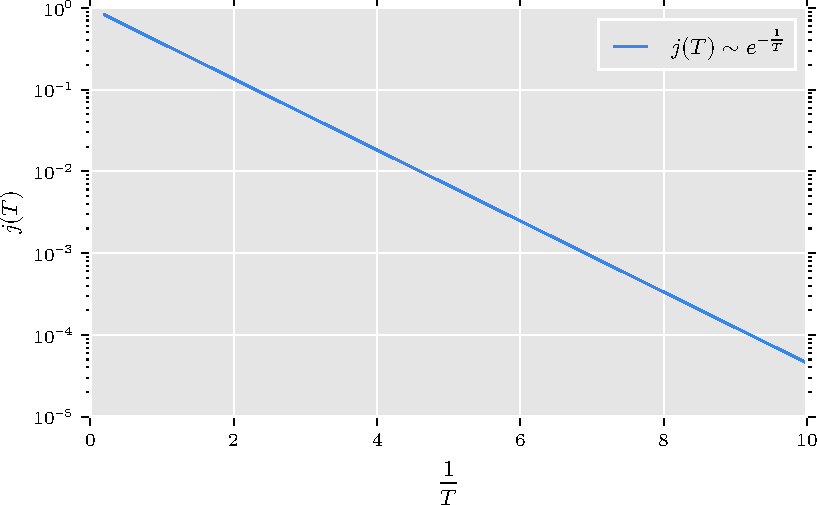
\includegraphics{strom.pdf}
  \caption{Verlauf der Funktion  $j(T) = e^{- \frac{1}{T}}$ }
\end{figure}

Die zweite Möglichkeit zur Messung der Aktivierungsenergie $W$ beutzt den gesamten Kurvenverlauf des gemessen Stroms.
Für die Gesamtpolarisation $P$ gilt Differentialgleichung \eqref{eq:pol}
